\chapter{Results and Discussion}
\justifying

This chapter presents the results of the four approaches on the common test set, analyses their errors, training behaviour and speed, and then answers the research questions.

\section{Overall Comparison}

Table~\ref{tab:main} summarises the performance of all four approaches, and Figure~\ref{fig:f1bar} compares their F1-scores.

\begin{table}[H]
  \centering
  \caption{Results on the test set (3,183 comments). Fine-tuned models: mean $\pm$ standard deviation over three runs. Precision, recall and F1 are weighted averages. Speed is comments per second.}
  \label{tab:main}
  \small
  \begin{tabular}{lccccr}
    \toprule
    \textbf{Model} & \textbf{Accuracy} & \textbf{Precision} & \textbf{Recall} & \textbf{F1} & \textbf{Speed} \\
    \midrule
    better\_profanity (lexicon) & 0.4684 & 0.2194 & 0.4684 & 0.2989 & 21.4 \\
    LLM, zero-shot (Qwen)$^{*}$ & 0.7748 & 0.8347 & 0.7748 & 0.7681 & 2.6 \\
    BanglaBERT (fine-tuned) & 0.9276 $\pm$ 0.0035 & 0.9279 & 0.9276 & 0.9276 $\pm$ 0.0035 & 183.3 \\
    \textbf{XLM-RoBERTa (fine-tuned)} & \textbf{0.9430 $\pm$ 0.0013} & \textbf{0.9433} & \textbf{0.9430} & \textbf{0.9430 $\pm$ 0.0013} & 177.2 \\
    \bottomrule
  \end{tabular}

  \vspace{0.2cm}
  \footnotesize $^{*}$Scored on the 3,033 of 3,183 test comments that it classified before the daily API limit was reached (Section~\ref{sec:llm}).
\end{table}

\begin{figure}[H]
  \centering
  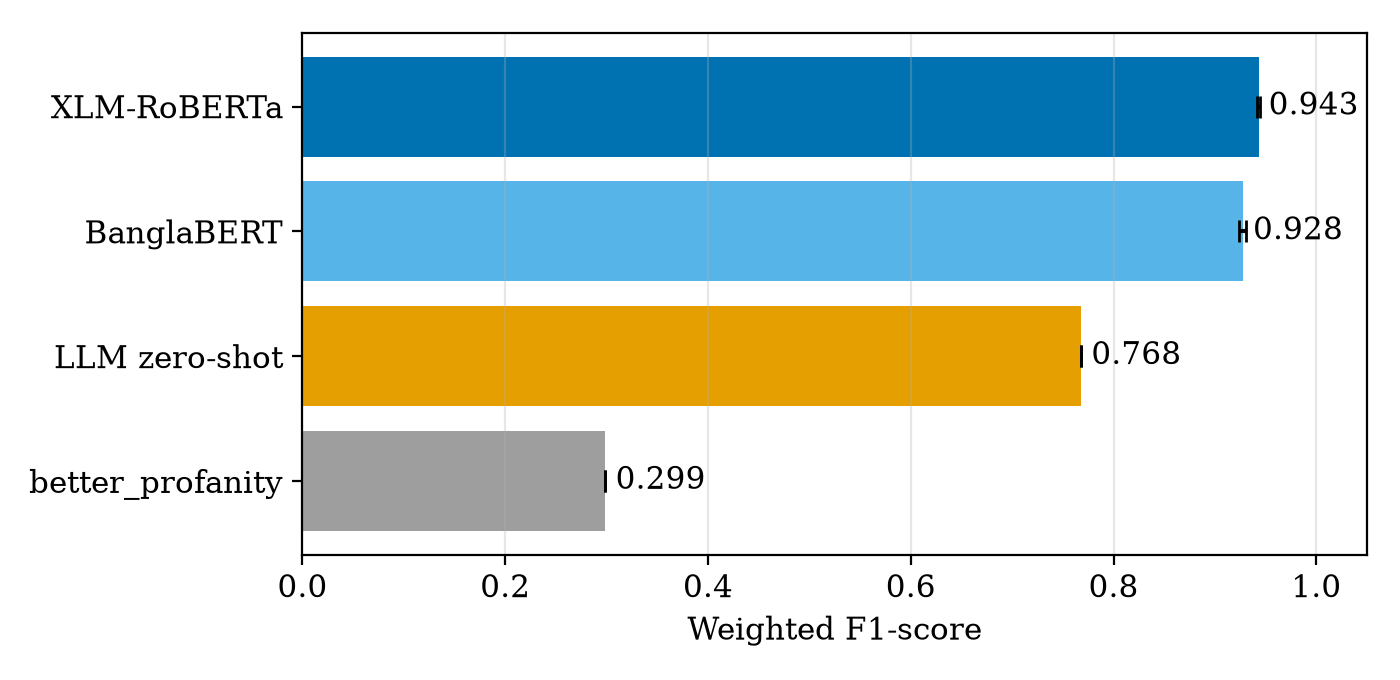
\includegraphics[width=0.85\textwidth]{f1_comparison.png}
  \caption{Weighted F1-score of each approach on the test set. Error bars show the standard deviation over three runs for the fine-tuned models.}
  \label{fig:f1bar}
\end{figure}

The fine-tuned transformers clearly outperform the other two approaches. XLM-RoBERTa is the best model, with an F1-score of 0.943, followed by BanglaBERT at 0.928. The zero-shot LLM is about 16 F1 points behind them, and the lexicon filter barely works. The sections below look at each approach in more detail.

\section{Lexicon Baseline}

The \texttt{better\_profanity} filter reaches an accuracy of 0.468 and an F1-score of 0.299. Its confusion matrix (Figure~\ref{fig:cm}) shows that it labelled every one of the 3,183 test comments as non-toxic, so its accuracy simply equals the share of non-toxic comments in the test set ($1{,}491/3{,}183 = 0.468$). The reason is that its word list contains English words, which almost never occur in Bangla script. This confirms that an off-the-shelf English profanity filter offers no protection for Bangla users, and that toxicity detection needs language-specific resources.

\section{Fine-tuned Transformer Models}

\subsection{Performance and Stability}

The F1-scores of the three BanglaBERT runs were 0.9270, 0.9236 and 0.9321 (mean 0.9276, standard deviation 0.0035). The three XLM-RoBERTa runs scored 0.9412, 0.9444 and 0.9433 (mean 0.9430, standard deviation 0.0013). The gap between the two models (about 1.5 F1 points) is more than four times the larger standard deviation, and every XLM-RoBERTa run scored higher than every BanglaBERT run. The difference is therefore consistent across random seeds, although three runs are too few for a formal significance test. XLM-RoBERTa is also the more stable of the two models. A training run took about 14 minutes for BanglaBERT and 17 minutes for XLM-RoBERTa on the T4 GPU.

\subsection{Error Analysis}

Figure~\ref{fig:cm} shows the confusion matrices of all four approaches, and Table~\ref{tab:perclass} gives per-class scores for the three approaches that detect toxicity at all.

\begin{figure}[H]
  \centering
  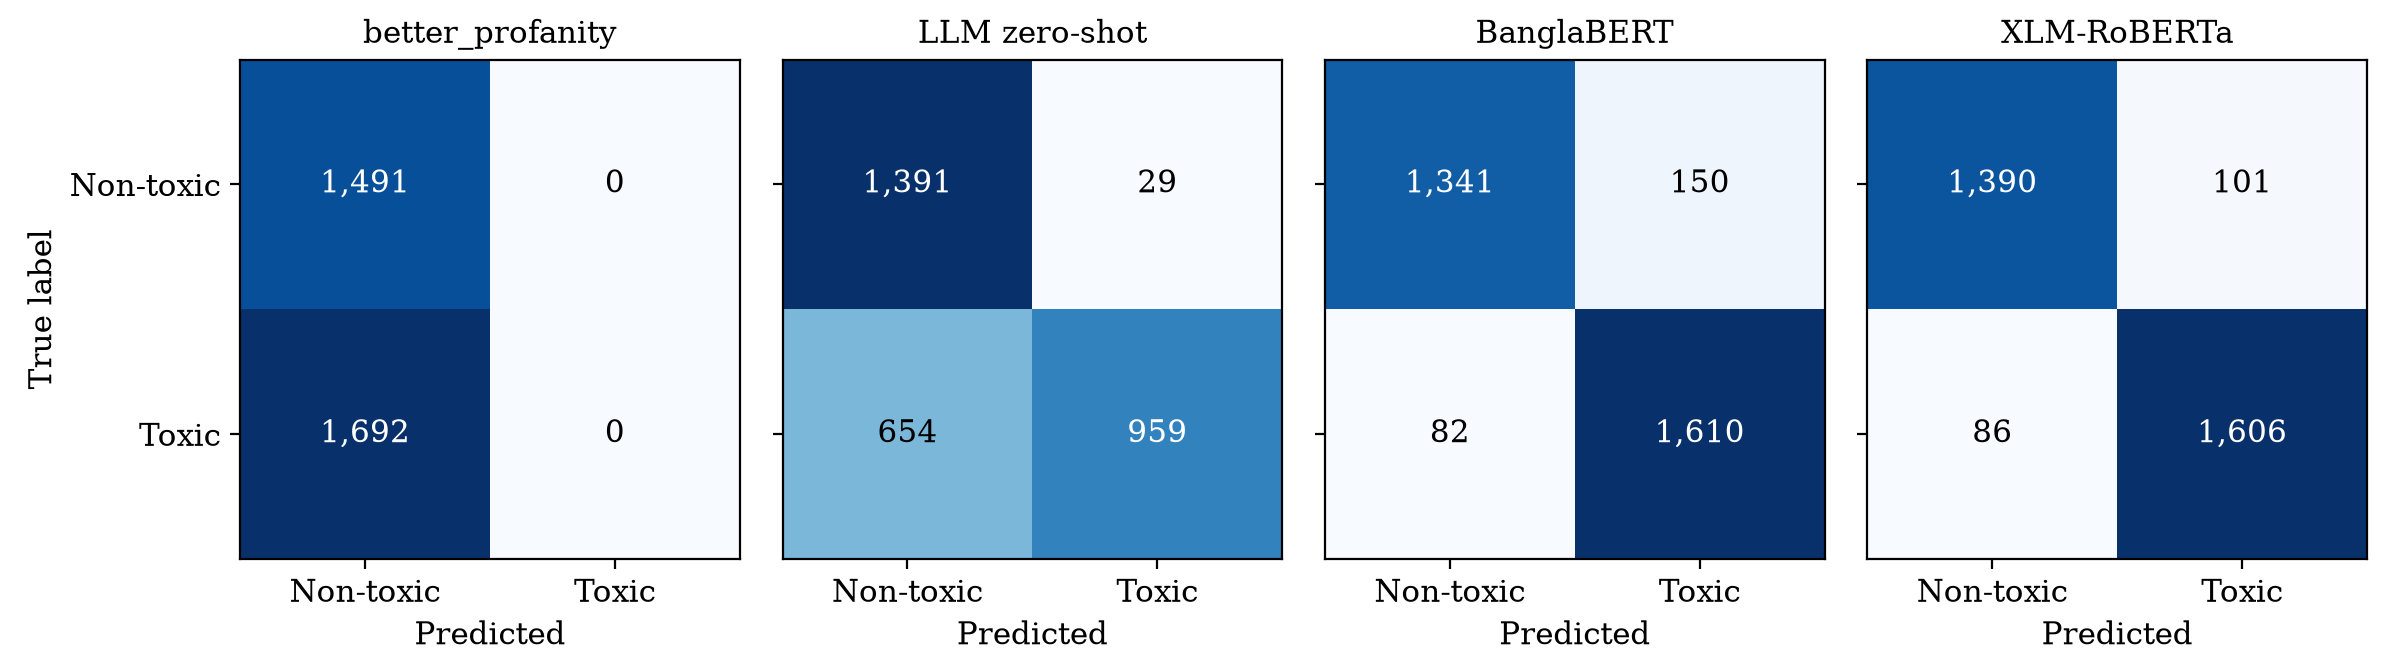
\includegraphics[width=\textwidth]{confusion_matrices.png}
  \caption{Confusion matrices on the test set (first run for the fine-tuned models). Rows are true labels, columns are predictions. The LLM matrix covers the 3,033 comments it classified.}
  \label{fig:cm}
\end{figure}

\begin{table}[H]
  \centering
  \caption{Per-class precision, recall and F1 on the test set, computed from the confusion matrices in Figure~\ref{fig:cm}.}
  \label{tab:perclass}
  \begin{tabular}{llccc}
    \toprule
    \textbf{Model} & \textbf{Class} & \textbf{Precision} & \textbf{Recall} & \textbf{F1} \\
    \midrule
    \multirow{2}{*}{BanglaBERT} & Non-toxic & 0.942 & 0.899 & 0.920 \\
                                & Toxic     & 0.915 & 0.952 & 0.933 \\
    \midrule
    \multirow{2}{*}{XLM-RoBERTa} & Non-toxic & 0.942 & 0.932 & 0.937 \\
                                 & Toxic     & 0.941 & 0.949 & 0.945 \\
    \midrule
    \multirow{2}{*}{LLM zero-shot} & Non-toxic & 0.680 & 0.980 & 0.803 \\
                                   & Toxic     & 0.971 & 0.595 & 0.737 \\
    \bottomrule
  \end{tabular}
\end{table}

The two fine-tuned models make different kinds of errors. BanglaBERT leans towards flagging comments: it misses only 82 of 1,692 toxic comments (4.8\%), but wrongly flags 150 of 1,491 non-toxic ones (10.1\%). XLM-RoBERTa misses a similar number of toxic comments (86, or 5.1\%) while raising a third fewer false alarms (101, or 6.8\%). Its advantage therefore comes mainly from recognising harmless comments more reliably. For a moderation system this matters, because every false alarm means a legitimate comment is hidden or sent for manual review.

\subsection{Training Dynamics}

Figure~\ref{fig:dynamics} shows the training and validation loss and the validation F1-score of a BanglaBERT training run over its five epochs. The training loss falls steadily from 0.26 to 0.03. The validation loss is lowest after the first epoch and then rises to 0.58, while the validation F1-score still improves slightly, from 0.903 to 0.914. The model therefore becomes increasingly over-confident on the examples it gets wrong (overfitting, as measured by the loss), even though the number of correct decisions keeps rising a little. Selecting checkpoints by validation F1 rather than validation loss is therefore appropriate for this task. Fewer epochs, or stronger regularisation, would likely give similar F1-scores at a lower training cost.

\begin{figure}[H]
  \centering
  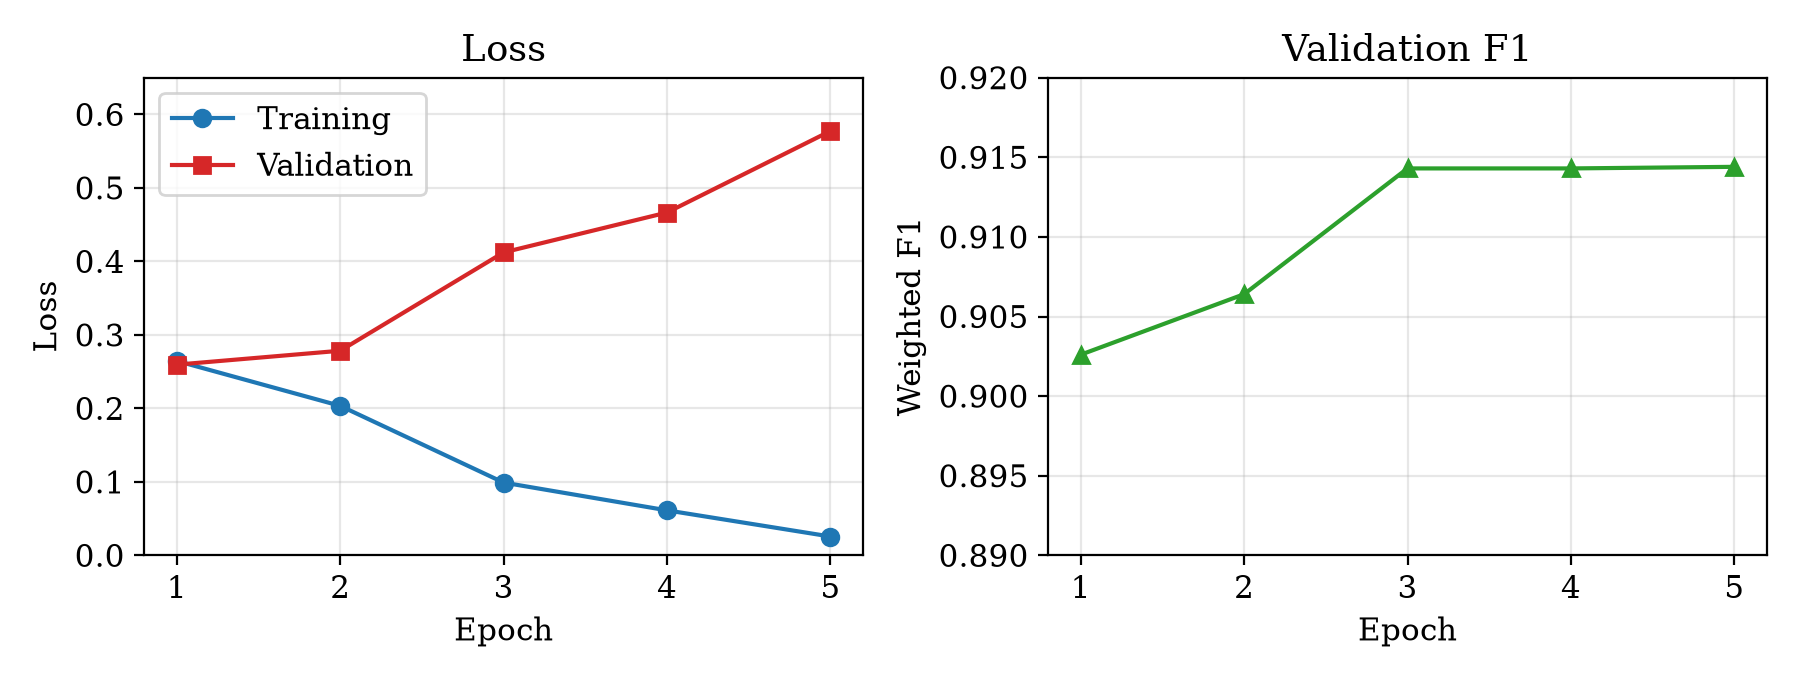
\includegraphics[width=\textwidth]{training_dynamics.png}
  \caption{Training behaviour of BanglaBERT over five epochs (seed 43). The validation loss rises after the first epoch, a sign of overfitting, while the validation F1-score still improves slightly.}
  \label{fig:dynamics}
\end{figure}

\subsection{Effect of Training Data Size}

Figure~\ref{fig:lc} shows the test F1-score when the models are trained on 25\%, 50\% and 100\% of the training data.

\begin{figure}[H]
  \centering
  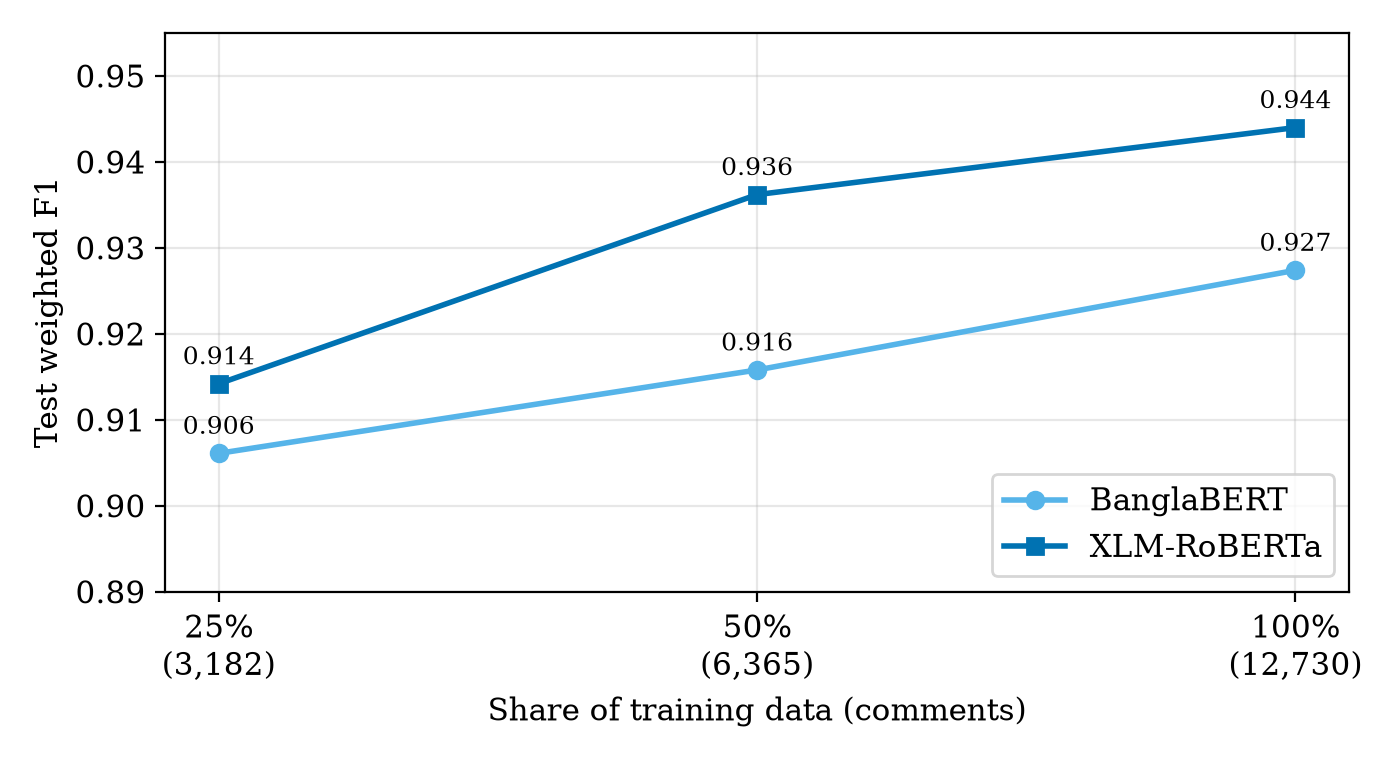
\includegraphics[width=0.85\textwidth]{learning_curves.png}
  \caption{Learning curves: test F1-score of each fine-tuned model against the amount of training data used.}
  \label{fig:lc}
\end{figure}

Three observations stand out. First, both models already perform well with little data: trained on only 3,182 comments (25\%), they reach F1-scores of 0.906 (BanglaBERT) and 0.914 (XLM-RoBERTa), far above the zero-shot LLM. Second, both curves are still rising at 100\%: going from half to all of the data adds 1.2 F1 points for BanglaBERT and 0.8 for XLM-RoBERTa. More labelled data would therefore probably still help, although with diminishing returns. Third, XLM-RoBERTa is ahead at every data size, and XLM-RoBERTa trained on half of the data (0.936) already outperforms BanglaBERT trained on all of it (0.927).

\section{Zero-shot LLM Baseline}
\label{sec:llm}

The LLM classified 3,033 of the 3,183 test comments. The remaining 150 comments (six batches) were not classified because the free tier of the API limits usage to 200,000 tokens per day \cite{groqdocs}. Because the test set is in random order, the missing comments are an essentially random subset, so excluding them should not bias the result noticeably. They are excluded from the LLM's scores rather than counted as errors.

The LLM reaches an F1-score of 0.768. Its behaviour is very different from that of the fine-tuned models (Table~\ref{tab:perclass}). When it labels a comment as toxic, it is almost always right: toxic precision is 0.971, with only 29 false alarms. However, it misses 654 of 1,613 toxic comments, a toxic recall of only 0.595. In other words, the model is very \emph{conservative}: it flags only clearly offensive comments and lets milder insults, trolling and implicit attacks through. Possible explanations include the model's limited exposure to informal Bangla, including slang and spelling variants, differences between the model's notion of toxicity and the dataset's annotation guidelines (which count trolling and mild insults as toxic), and the absence of any examples in the prompt.

The LLM is also slow in this setup: 2.6 comments per second, compared with about 180 for the fine-tuned models. Classifying the full test set took roughly 20 minutes and used almost the entire daily free-tier allowance, and the approach depends on an external service. These factors make zero-shot prompting impractical for large-scale moderation, although it may still be useful as a quick, high-precision first filter where no labelled data is available.

\section{Inference Efficiency}

Figure~\ref{fig:speed} plots accuracy against speed. The fine-tuned models are both the most accurate and the fastest. They classify about 180 comments per second on a single free GPU, roughly 70 times faster than the LLM. Once trained, they also run without any external service or per-request cost. The lexicon filter is relatively slow, at 21 comments per second, probably because it checks every word against its list in pure Python.

\begin{figure}[H]
  \centering
  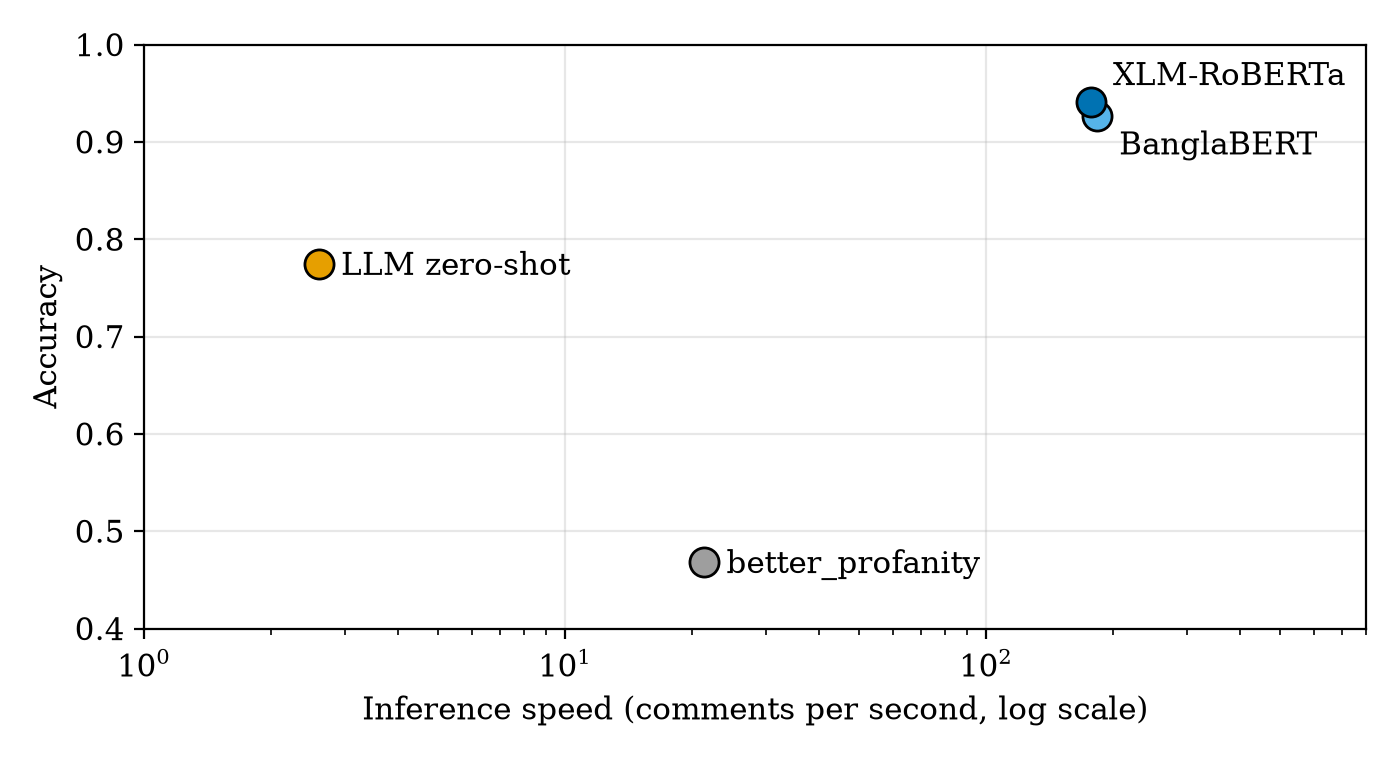
\includegraphics[width=0.85\textwidth]{accuracy_vs_speed.png}
  \caption{Accuracy against inference speed. The fine-tuned models are both the most accurate and the fastest. Fine-tuned model accuracy is from the first run.}
  \label{fig:speed}
\end{figure}

\section{Comparison with Previous Work}

Belal et al. \cite{belal2023toxic} reported a binary toxic-versus-non-toxic accuracy of 89.42\% on the same dataset. The fine-tuned models in this thesis reach a mean accuracy of 92.8\% (BanglaBERT) and 94.3\% (XLM-RoBERTa). The results are not directly comparable, because the train/test splits, preprocessing (this thesis removes duplicate comments) and evaluation details differ. Nevertheless, they indicate that fine-tuning modern pretrained transformers is a strong approach for this dataset.

\section{Answers to the Research Questions}

\textbf{RQ1: How accurately can fine-tuned transformers detect toxic Bangla comments?} Very accurately. Both models exceed an F1-score of 0.92 and miss only about 5\% of toxic comments, and their results vary little between runs.

\textbf{RQ2: Does the Bangla-specific model outperform the multilingual one?} No. XLM-RoBERTa outperforms BanglaBERT by about 1.5 F1 points, consistently across seeds and at every training-data size, mainly by raising fewer false alarms. A likely explanation is that XLM-RoBERTa was pretrained on far more data overall (2.5 TB of filtered web text) and has a larger vocabulary, so it may have seen more of the informal, varied language found in social-media comments. The result shows that being language-specific does not by itself guarantee better performance, although a larger Bangla model such as \texttt{csebuetnlp/banglabert} \cite{bhattacharjee2022banglabert} may close the gap.

\textbf{RQ3: How does a zero-shot LLM compare?} It is clearly worse, with an F1-score of 0.768 against 0.928--0.943. It is very precise but misses about 41\% of toxic comments, and it is about 70 times slower in this setup. Fine-tuning on a few thousand labelled examples remains the better choice when labelled data is available.

\textbf{RQ4: Is a lexicon filter adequate?} No. An off-the-shelf English profanity filter did not flag a single toxic comment in the Bangla test set.

\textbf{RQ5: How does performance depend on training data size?} Performance rises steadily with more data, but even a quarter of the training set (about 3,200 comments) gives F1-scores above 0.90. The curves have not flattened at 12,730 comments, so collecting more labelled data would probably bring further, smaller gains.
